\documentclass[spanish]{beamer}

%%% CODIFICACIÓN

%\usepackage[x11names, rgb, html]{xcolor}
\usepackage[utf8]{inputenc}
\usepackage[spanish]{babel}
\usepackage{graphics}

%%% FUENTES

\usepackage[T1]{fontenc}
\usepackage[familydefault,regular]{Chivo}
\usepackage{newtxsf} % Fuente de matemáticas
\usepackage{mathastext}
\usepackage[scaled=.85]{FiraMono}

\setbeamertemplate{navigation symbols}{}

%%% COLORES

\definecolor{50}{HTML}{FFEBEE}
\definecolor{100}{HTML}{FFCDD2}
\definecolor{200}{HTML}{EF9A9A}
\definecolor{300}{HTML}{E57373}
\definecolor{400}{HTML}{EF5350}
\definecolor{500}{HTML}{F44336}
\definecolor{600}{HTML}{E53935}
\definecolor{700}{HTML}{D32F2F}
\definecolor{800}{HTML}{C62828}
\definecolor{900}{HTML}{B71C1C}

%% Colores de Solarized

\definecolor{sbase03}{HTML}{002B36}
\definecolor{sbase02}{HTML}{073642}
\definecolor{sbase01}{HTML}{586E75}
\definecolor{sbase00}{HTML}{657B83}
\definecolor{sbase0}{HTML}{839496}
\definecolor{sbase1}{HTML}{93A1A1}
\definecolor{sbase2}{HTML}{EEE8D5}
\definecolor{sbase3}{HTML}{FDF6E3}
\definecolor{syellow}{HTML}{B58900}
\definecolor{sorange}{HTML}{CB4B16}
\definecolor{sred}{HTML}{DC322F}
\definecolor{smagenta}{HTML}{D33682}
\definecolor{sviolet}{HTML}{6C71C4}
\definecolor{sblue}{HTML}{268BD2}
\definecolor{scyan}{HTML}{2AA198}
\definecolor{sgreen}{HTML}{859900}

%% Colores del documento

\definecolor{background}{RGB}{237,237,237}
\definecolor{text}{RGB}{78,78,78}
\definecolor{accent}{RGB}{129, 26, 24}
\definecolor{accent2}{HTML}{814918}
\definecolor{accent3}{HTML}{136618}
\definecolor{accent4}{HTML}{0F4B4E}
\definecolor{accent5}{HTML}{681341}
\definecolor{accent6}{HTML}{1F1B5A}

\setbeamerfont{framesubtitle}{size=\normalfont\small}
\setbeamercolor{framesubtitle}{fg=white}

%%% AJUSTES DE BEAMER

\setbeamertemplate{frametitle}{\color{900}\vspace*{1cm}\insertframetitle\\\usebeamerfont{framesubtitle}\insertframesubtitle\par\vskip-6pt}

\setbeamertemplate{itemize items}[circle] % Viñetas de itemize

%%% CONFIGURACIÓN DE COLORES DE BEAMER

\setbeamercolor{background canvas}{bg=background}
\setbeamercolor{normal text}{fg=text}
\setbeamercolor{alerted text}{fg=900}
\setbeamercolor{block title}{fg=900}
\setbeamercolor{alerted text}{fg=900}
\setbeamercolor{itemize item}{fg=900}
\setbeamercolor{enumerate item}{fg=900}
\setbeamercolor*{title}{fg=900}
\setbeamercolor{qed symbol}{fg=900}
\usebeamercolor[fg]{normal text}

%%% INFORMACIÓN DEL DOCUMENTO

\title{Fundamentos de Redes}
\subtitle{Redes anónimas: I2P}
\author{Alberto Jesús Durán López\\ Antonio Coín Castro\\ \vspace{1em}Grupo 5}
\begin{document}


\maketitle



\begin{frame}{Privacidad en la red}
	
	\textit{"[Privacy] can be defined as an individual's claim to control the terms under which personal information -- information identifiable to the individual -- is acquired, disclosed, and used."}

	
\end{frame}



\begin{frame}{Anonimato en el acceso corriente a Internet}

\begin{itemize}
	\item Identificación de forma unívoca por la \textbf{dirección IP}
	\item Geolocalización
    \item Rastreo de datos personales (\textit{tracking})\\ 
    \item Cookies
    \item Anuncios dirigidos
\end{itemize}

\end{frame}  



\begin{frame}{Métodos para mantener el anonimato}
	
\begin{itemize}
	\item Proxy \\
	\item VPN\\ 
	\item Redes anónimas\\
	\item Otros
\end{itemize}	
	
\end{frame}



\begin{frame}{Proxy}
	
Servidor intermediario entre las conexiones de un cliente y un servidor. \\

\begin{figure}[h]
 	\centering
 	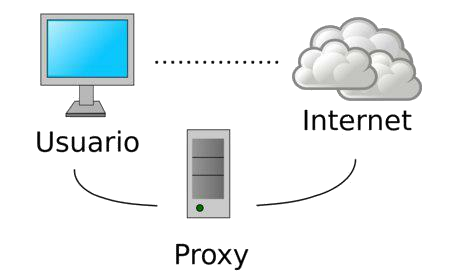
\includegraphics[width=.5\textwidth]{img/proxy}
\end{figure}


\begin{itemize}
	\item Dirección IP camuflada \\
	\item Acceso a contenido bloqueados en algunos países \\ 
\end{itemize}
	
\end{frame}

\begin{frame}{VPN}
 	\begin{figure}[h]
 		\centering
 		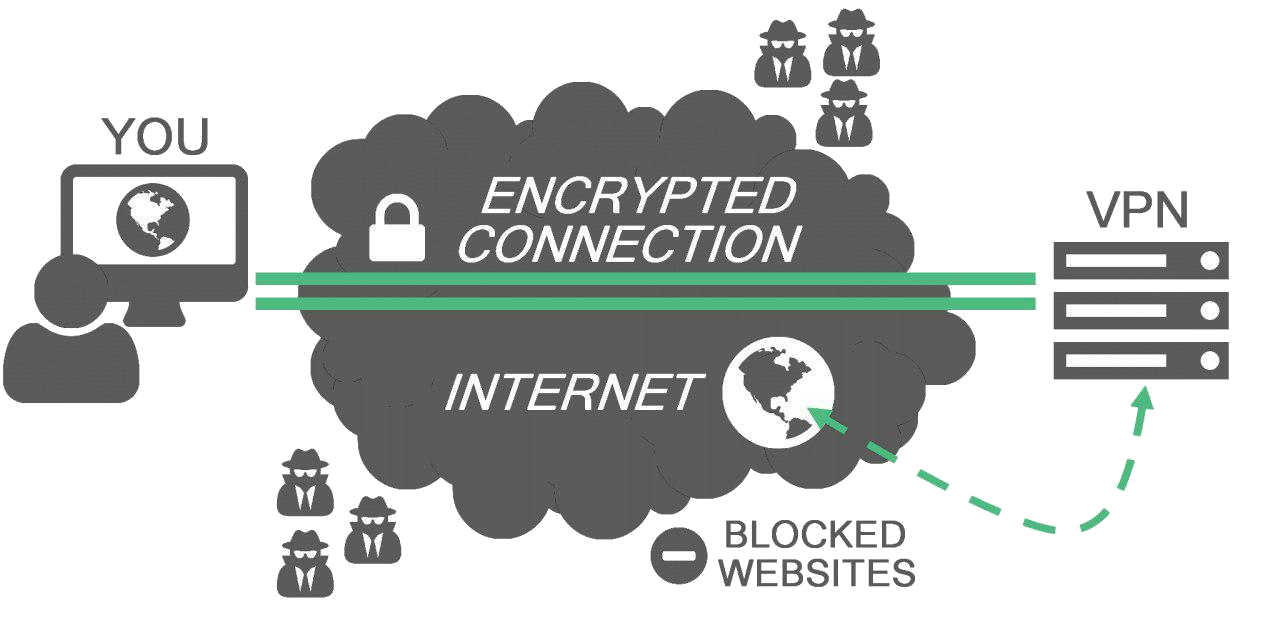
\includegraphics[width=.75\textwidth]{img/vpn}
 	\end{figure}
 \end{frame}

\begin{frame}{VPN}

Acrónimo de \textit{Virtual Private Network}. Es un medio de extender una red privada a través de una red pública.

\vspace{1.9em}

\begin{itemize}
	\item Acceso remoto a una red privada (UGR) \\
	\item Dirección IP camuflada \\ 
	\item Confidencialidad garantizada: paquetes encriptados \\
	\item Sistema de autentificación para conectarse
	\item Mecanismos para mantener integridad de mensajes
\end{itemize}	

\end{frame}



\begin{frame}{Otros$\dots$}

\begin{itemize}
	\item Buscadores que no te rastrean (e.g. DuckDuckGo)
	\item Sistemas operativos específicos (e.g. Tails)
\end{itemize}

\end{frame}



\begin{frame}{Redes anónimas}{Invisible Internet Project}
	\vspace{-1em}
	
	\begin{figure}
	\centering
	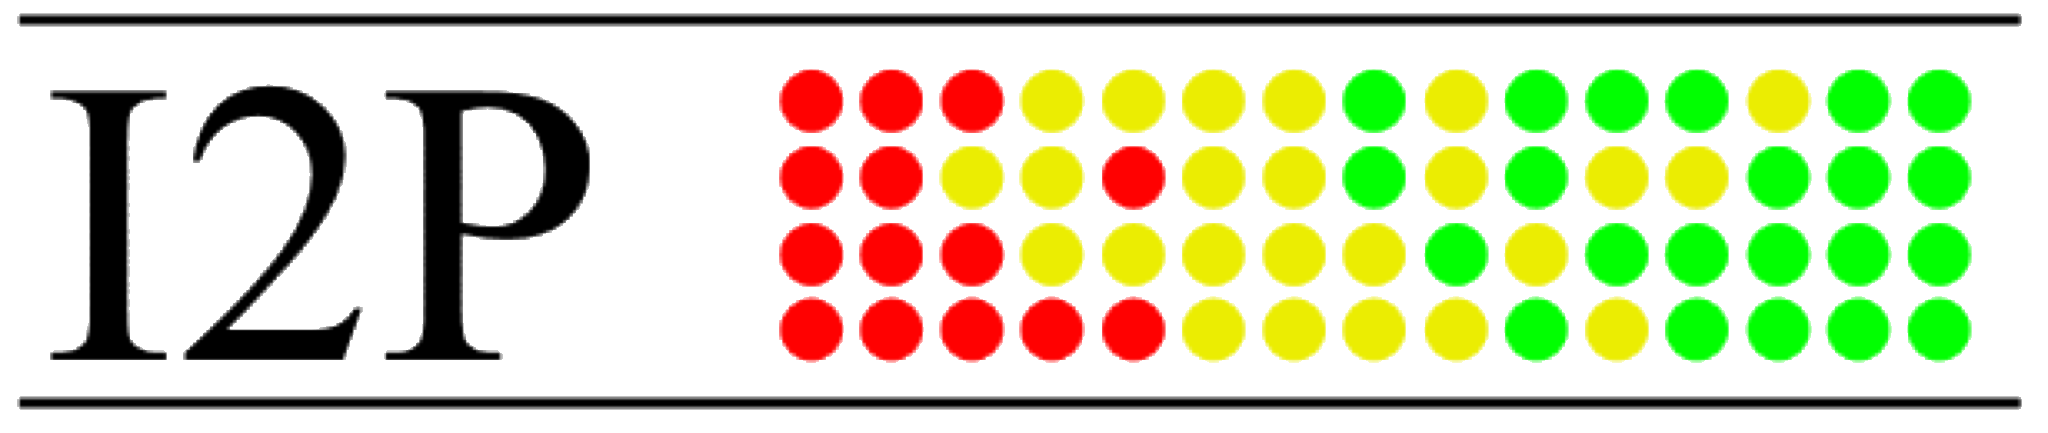
\includegraphics[width=.5\textwidth]{img/i2p_logo}
\end{figure}
I2P es una herramienta de \textbf{software libre} que ofrece una capa de red de abstracción distribuida para comunicaciones entre ordenadores, la cual permite a las aplicaciones que la utilizan transmitir mensajes de forma anónima y segura.
	
\end{frame}



\begin{frame}{Invisible Internet Project}{Estructura}

Se trata de una red superpuesta (\textit{overlay network}) basada en el intercambio de paquetes.

\begin{itemize}
	\item Los paquetes están dirigidos a direcciones criptográficas.
	\item Emisor y receptor no pueden identificarse mutuamente.
	\item Comunicaciones ocultas a terceros (encriptadas).
	\item Funcionamiento P2P.
\end{itemize}
	
\end{frame}



\begin{frame}{Invisible Internet Project}{Estructura}

\begin{itemize}
\item Un \textbf{router} es un ordenador conectado a I2P. En general, nos referiremos a ellos también como \textbf{nodos} de la red.
\item Un \textbf{túnel} es una secuencia de nodos que forman camino temporal, unidireccional y seguro por el que viajan los mensajes.
\end{itemize}

	
\end{frame}



\begin{frame}{Invisible Internet Project}{Funcionamiento}

Cada cliente construye una serie de túneles de entrada (\textit{inbound}) y de salida (\textit{outbound}). El primer nodo de un túnel se denomina \textit{gateway}.


\begin{figure}
	\centering
	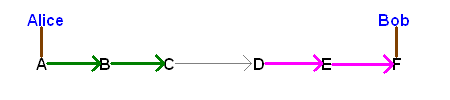
\includegraphics[width=.7\textwidth]{img/alice_bob_tunnel}
\end{figure}

Se elige la longitud del túnel para encontrar un equilibrio entre el anonimato, la latencia y el \textit{throughput}.

\end{frame}

\begin{frame}{Invisible Internet Project}{netDB}

La base de datos en red está completamente distribuida. En cada instante, hay un subconjunto de nodos especiales (\textit{floodfill nodes}) encargados de mantenerla.\\

\begin{figure}
	\centering
	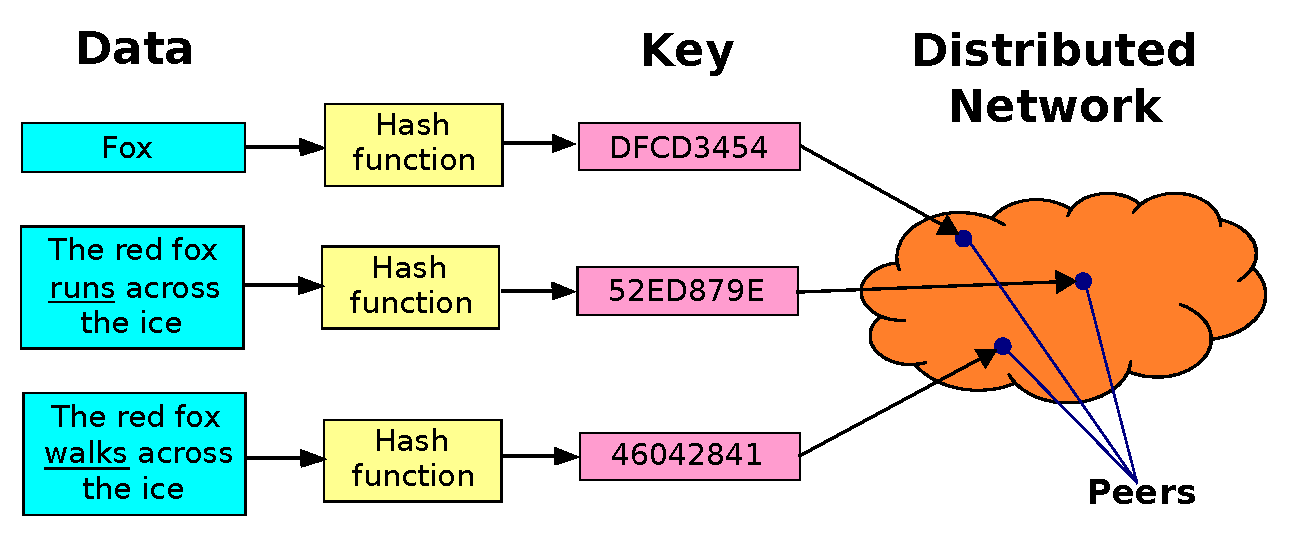
\includegraphics[width=.6\textwidth]{img/DHT.pdf}
\end{figure}

Cuando se envía un mensaje, se buscan en la tabla los túneles de entrada del nodo destino (\textit{LeaseSet}).
\end{frame}

\begin{frame}{Invisible Internet Project}{netDB}
	La información que se almacena en la tabla es la siguiente:
	\vspace{1.5em}
	
	\begin{itemize}
	\item \textbf{RouterInfo:} estructura que contiene información para contactar a un router concreto.
	\item \textbf{LeaseSet:} información para establecer comunicación con un destino concreto (otro nodo, un servidor de correo, un sitio web$\dots$).
\end{itemize}
\end{frame}

\begin{frame}{Invisible Internet Project}{Algoritmo Kademlia}

Los accesos y consultas a la base de datos se realizan al nodo \textit{floodfill} más cercano. La medida de cercanía se computa utilizando la métrica XOR sobre el ID de los nodos.

\vspace{1.5em}
\begin{itemize}
	\item $A \oplus B \ge 0$, y $A \oplus B = 0 \iff A = B$ 
	\item $A \ \oplus \ B = B \ \oplus \ A$.
	\item $A \oplus B \leq (A \ \oplus \ C) + (C \ \oplus \ B)$
\end{itemize}
	
\end{frame}


\begin{frame}{Invisible Internet Project}{Ejemplo de comunicación}
\begin{figure}
	\centering
	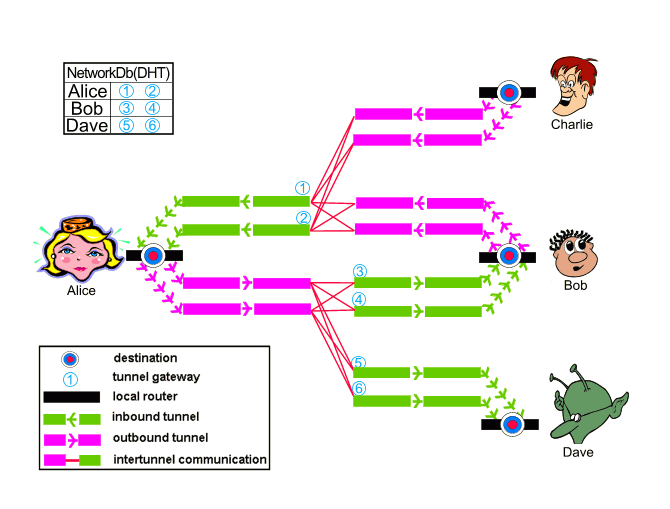
\includegraphics[width=.8\textwidth]{img/alice_bob_message}
\end{figure}
	
\end{frame}


\begin{frame}{\textit{Garlic routing}}
	
Enrutamiento tipo garlic:


\begin{itemize}
	\item Cifrado por capas
	\item Agregación de múltiples mensajes juntos
	\item Cifrado ElGamal/AES
\end{itemize}
	
\end{frame}


\begin{frame}{\textit{Garlic routing}}{Cifrado por capas}
	
 
 
 \begin{itemize}
 	\item Comunicación de dos usuarios mediante túneles
 	\item La información viaja desde el primer nodo del túnel hasta el último
 	\item El '\textit{gateway}' fragmenta mensajes I2P en mensajes de túnel
 	\item En cada salto se envía: \{ID del túnel, IV, mensaje del túnel\}
 \end{itemize}
 
 
 \end{frame}
 
 
 \begin{frame}{\textit{Garlic routing}}{Agregación de mensajes}
 
 
 Agregación de múltiples mensajes juntos juntos para aumentar velocidad de transferencia de datos y aumentar seguridad.
 
 \begin{figure}
\centering
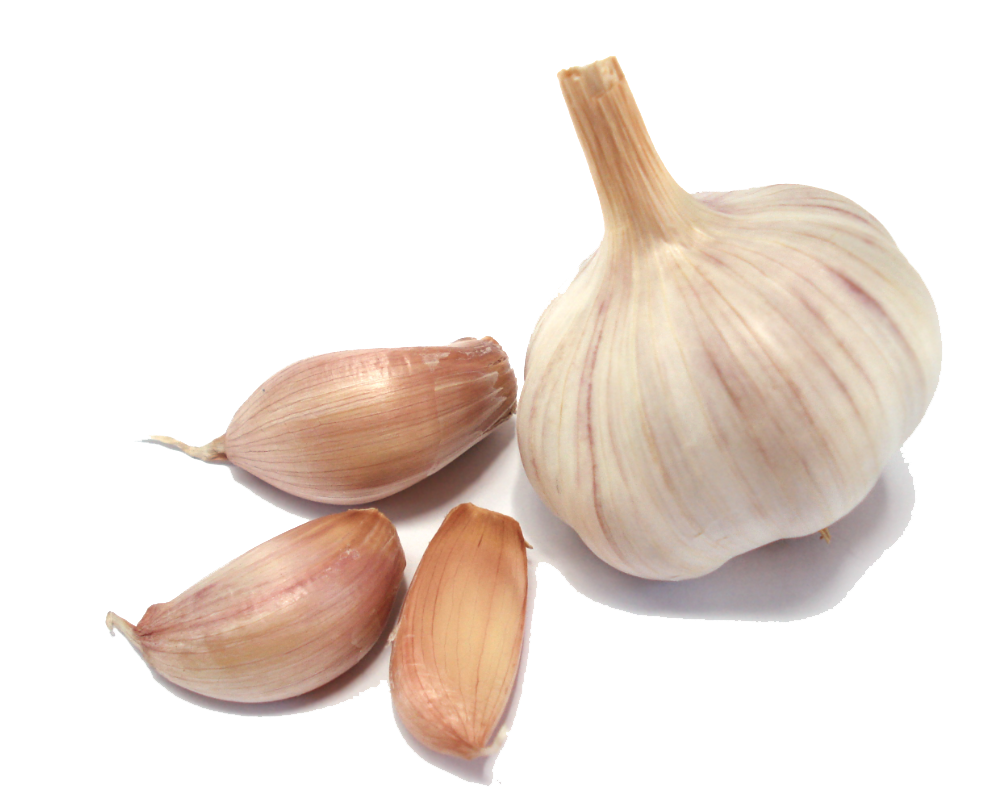
\includegraphics[width=.35\textwidth]{img/garlic}
\end{figure}

 	
 \end{frame}
 
 \begin{frame}{\textit{Garlic routing}}{Encriptación de la información}
 
 Tipos de cifrado:
 \begin{itemize}
 	\item Cifrado ElGamal
 	\item AES: Cifrado simétrico por bloques de 128 bits
 \end{itemize}
 \vspace{1em}
 
 Procedimiento aplicado a los mensajes:
 	\begin{itemize}
 		\item Se cifra el IV recibido con AES
 		\item Usa el IV obtenido para cifrar los datos
 		\item Cifra de nuevo el IV usando AES
 		\item Envía \{ID del túnel, IV, mensaje del túnel\} al siguiente nodo
 	\end{itemize}

 
 \end{frame}
 
 
 
 \begin{frame}{I2P vs Tor}
 
 \begin{itemize}
	\item \textit{Onion routing} vs \textit{Garlic routing}
	\item \textit{Túneles bidireccionales vs túneles unidireccionales}
	\item Directorio distribuido vs centralizado. Peer selection.
	\item Outproxies
\end{itemize}
   
\end{frame}
 
 
 \begin{frame}{Software I2P}
 	
 
 \begin{itemize}
 	\item Susimail: Interfaz web  para emails
 	\item Syndie: blogs, noticias y foros para I2P
 	\item I2P Messenger: Cliente de mensajería instantánea
 	\item Navegación web mediante webs anónimas
 	\item Compartición de archivos mediante el uso de BitTorrent dentro de la red I2P
 	\item (Android) Nightweb, aplicación que usa I2P y BitTorrent para compartir entradas
 	de blogs, fotos y otros contenidos similares
 \end{itemize}
 	
 \end{frame}

\begin{frame}{I2P}{Demo}
Acceso a la red I2P. Configuración, panel de control y ejemplo de navegación.\\

\vspace{2em}

El software se puede descargar en el siguiente enlace: \href{https://geti2p.net/en/download}{\url{https://geti2p.net/en/download}}
	
\end{frame}

\end{document}
